
\documentclass{report}
\usepackage{listings} % Pacote para destacar códigos
\usepackage{xcolor}
\usepackage{enumitem}
\usepackage{graphicx}
\usepackage[a4paper, total={6in, 9in}]{geometry}

\definecolor{linecolor}{RGB}{150,150,150}

\pagenumbering{gobble}

\lstset{
    basicstyle=\footnotesize,
    frame=tb,
    xleftmargin=0.2\textwidth,
    xrightmargin=0.2\textwidth,
}
\begin{document}


\huge

\centerline {Atividade Prática I} 
\centerline {Organização de Computadores I} 

\large

\bigskip

\centerline {Gabriel Salmoria e Gustavo Nunes Viana} 

\begin{itemize}
    
  \bigskip
    \item Atividade 1: 
      
Realizar as seguintes operações:

\skip
$$ a = b + 35; $$ 
$$ c = d - a + e; $$ 
\bigskip
Resolução:

\bigskip
Primeiramente, definimos as variáveis que iremos utilizar
para os valores de A, B, C, D e E. Para isso, vamos utilizar
a keyword ".word" para registrar os valores em algum local 
desconhecido na memória.
\\

\normalsize

\begin{lstlisting}[language=Ant]
        .data
          A: .word 0
          B: .word 25
          C: .word 0
          D: .word 10
          E: .word 20
\end{lstlisting}
\large

Depois, iremos carregar os ENDEREÇOS das variáveis que
iremos utilizar. Para isso, utilizaremos da pseudo-instrução
"load address", que irá carregar o endereço das variáveis definidas
anteriormente em registradores temporários.


\normalsize
\bigskip

\begin{lstlisting}[language=Ant]
          .text
            la $t0, A
            la $t1, B
            la $t2, C
            la $t3, D
            la $t4, E
            
\end{lstlisting}

\large

Após carregar os endereços, iremos carregar os VALORES das
variáveis. Para tal, faremos uso da instrução "Load Word", que
irá carregar os valores verdadeiros das variáveis nos registradores
source.

\normalsize
\bigskip

\begin{lstlisting}[language=Ant]
          lw $s0, 0($t0)
          lw $s1, 0($t1)
          lw $s2, 0($t2)
          lw $s3, 0($t3)
          lw $s4, 0($t4)
\end{lstlisting}


\large

Finalmente, iremos realizar as operações matemáticas. Primeiro
iremos calcular a expressão:

$$ a = b + 35; $$ 

Utilizando da instrução Adição imediata, ou Addi. Iremos passar
os valores de A (registrador s0), B (registrador s1) e o valor
imediato 35.

\normalsize
\bigskip

\begin{lstlisting}[language=Ant]
                addi $s0, $s1, 35
\end{lstlisting}


\large

Depois disso, iremos calcular a expressão:

$$ c = d - a + e; $$ 

Para isso, iremos realizar duas operações:

$$ c = d - a; $$ 
$$ c = c + e; $$ 

Tal expressão deve ser quebrada em duas pela natureza
das instruções matemáticas do Assembly, na qual, não
podemos ter mais que três variáveis envolvidas na mesma
operação.

\normalsize
\bigskip

\begin{lstlisting}[language=Ant]
          sub $s2, $s3, $s0;
          add $s2, $s2, $s4;
\end{lstlisting}


\large

Por fim, desejamos guardar o resultado das operações na
memória de dados, para isso, iremos utilizar a instrução
Store Word, ou sw.


\normalsize
\bigskip

\begin{lstlisting}[language=Ant]
		sw $s2, 0($t2)
\end{lstlisting}

\large


   \item Atividade 2:

     Adaptar a Atividade 1 para que o valor de B seja fornecido
     pelo usuário, e o valor de C seja apresentado no terminal
     além de ser salvo na variável B
  
  \bigskip
  Resolução:
  \bigskip
  
  Nessa questão, o nosso desafio está em interagir com o sistema
  operacional tanto para receber o valor de B quanto para mostrar
  o valor de C. Para isso, iremos utilizar a função syscall,
  inicialmente vamos passar o valor 5, para receber o valor digitado
  pelo usuário.


\normalsize
\bigskip

\begin{lstlisting}[language=Ant]
	li $v0, 5
	syscall
	move $s1, $v0

\end{lstlisting}

\large

Além disso, iremos utilizar, ao fim do programa, a função syscall
novamente, para mostrar o valor de C no terminal. Para isso, vamos
passar o valor 1:

\normalsize
\bigskip

\begin{lstlisting}[language=Ant]
	li $v0, 1
	add $a0, $a0, $s2
	syscall
\end{lstlisting}

\bigskip
\bigskip

\normalsize 

No nosso código da Atividade 1 há 19 linhas de instrução, sem contar pseudo-instruções

Ao fim de uma execução completa, esse é o resultado do programa:
\begin{figure}[h]
  \centering
  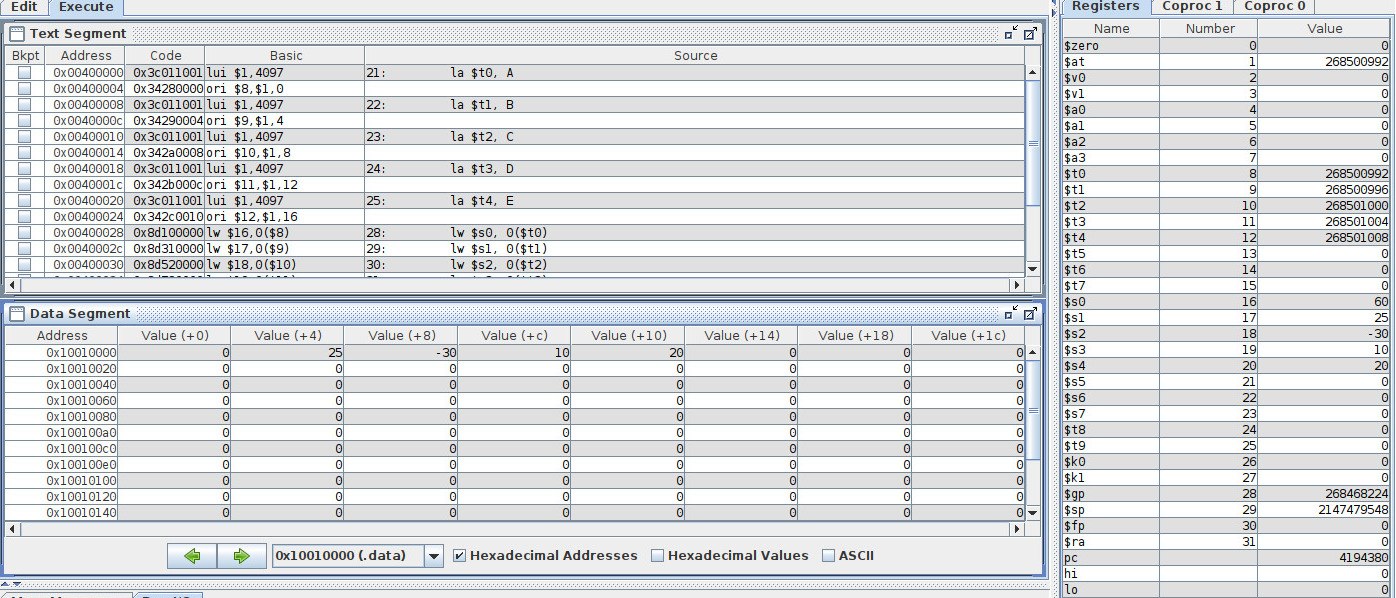
\includegraphics[width=1\textwidth]{exer1.jpeg}
\end{figure}



No nosso código da Atividade 2 há 21 linhas de instrução, sem contar pseudo-instruções

Ao fim de uma execução completa, esse é o resultado do programa:
\begin{figure}[h]
  \centering
  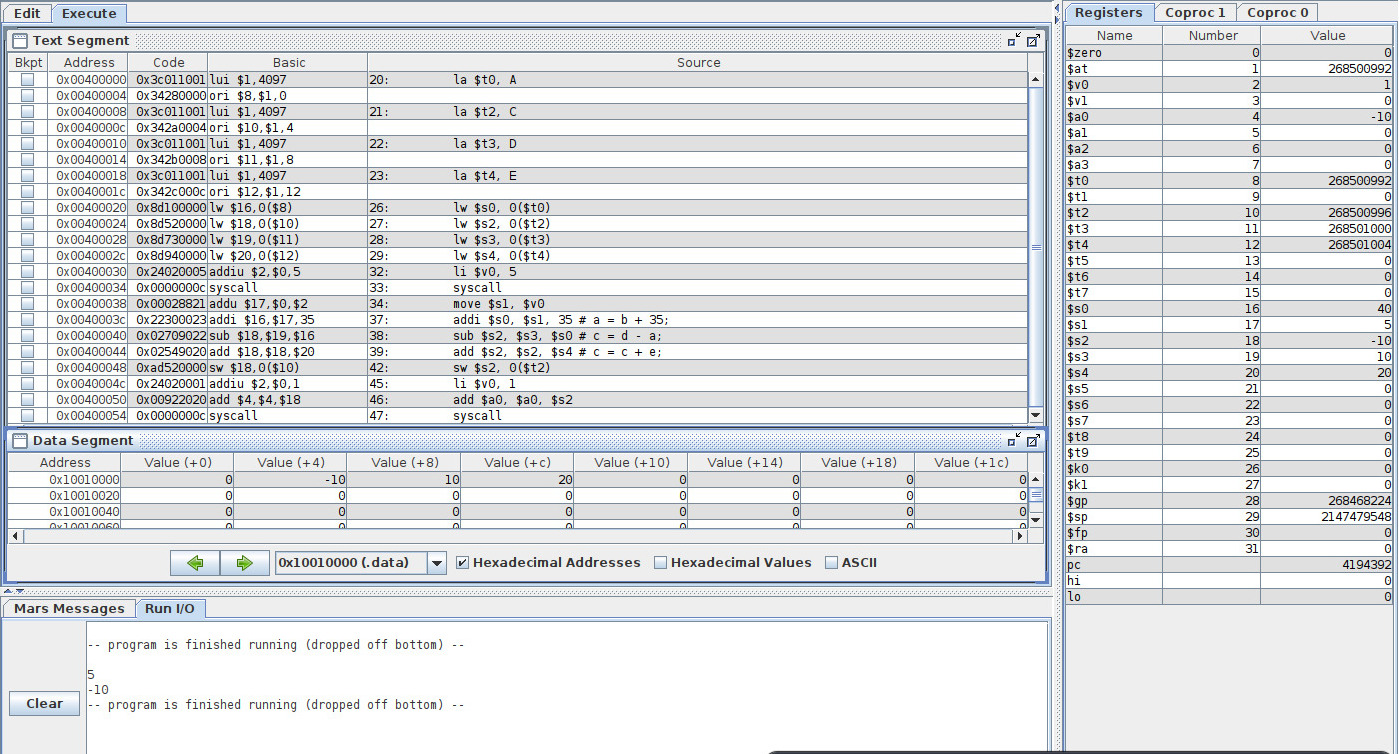
\includegraphics[width=1\textwidth]{exer2.jpeg}
\end{figure}


\end{itemize}

\end{document}
